\hypertarget{a00066}{\subsection{Com\-Objects.\-Msg\-Selection\-Request Klassenreferenz}
\label{a00066}\index{Com\-Objects.\-Msg\-Selection\-Request@{Com\-Objects.\-Msg\-Selection\-Request}}
}
Klassendiagramm für Com\-Objects.\-Msg\-Selection\-Request\-:\begin{figure}[H]
\begin{center}
\leavevmode
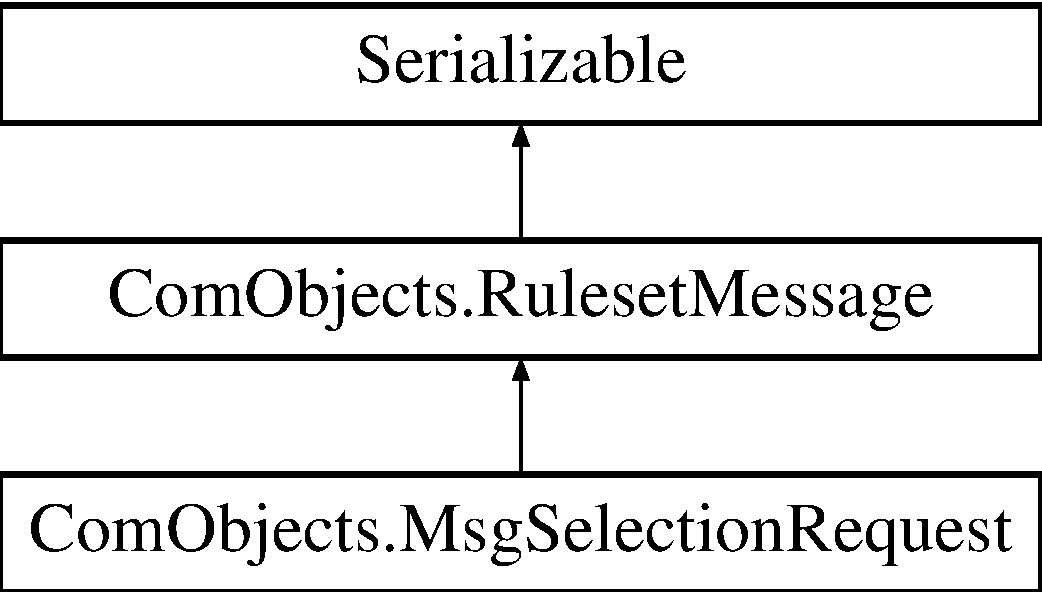
\includegraphics[height=3.000000cm]{a00066}
\end{center}
\end{figure}


\subsubsection{Ausführliche Beschreibung}
Diese Nachricht sendet der Server an einen Spieler, wenn er eine Auswahl von diesem erwartet. 